\documentclass[../report.tex]{subfiles}
\graphicspath{{\subfix{../images/}}}

\begin{document}
\section{Results}

For our simulation we have chosen the following parameters:
\begin{itemize}
    \item \textbf{Number of nodes}: Ranging from 2 to 200.
    \item \textbf{Simulation area}: A square area with side lengths varying from 1 to 200 units.
    \item \textbf{Number of packets sent}: Each node transmits 3 packets.
    \item \textbf{Simulation duration}: The total runtime is set to 10 seconds.
\end{itemize}

The \textbf{primary} performance \textbf{metric} analyzed in this study is the \textbf{number of lost packets} for each network configuration. The results indicate that as the number of nodes increases, the packet loss rate exhibits a non-linear trend. 

For \textbf{smaller networks} with a limited number of nodes, packet loss remains relatively \textbf{low} due to reduced congestion and simpler routing paths.

However, as \textbf{network area size increases}, a \textbf{higher} number of lost packets is observed, primarily attributed to \textbf{packet loss} caused by \textbf{nodes being too far apart} from each other, preventing effective communication and leading to dropped packets. Additionally, for networks containing a larger number of nodes, packet loss can be caused by increased contention, collisions, and routing inefficiencies in denser topologies.


\begin{figure}[H]
    \centering
    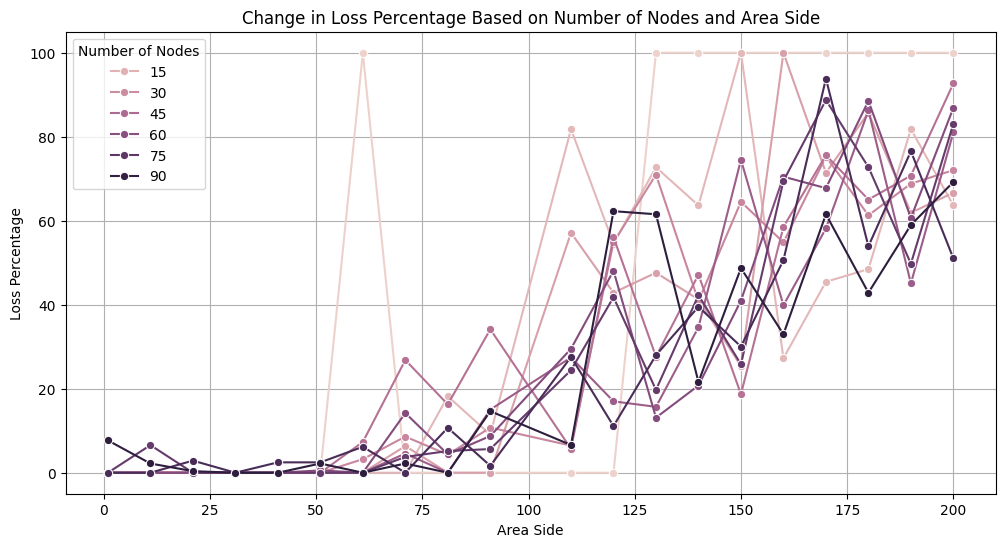
\includegraphics[width=1\linewidth]{images/loss_by_area.png}
    \caption{Change in Loss Percentage Based on Number of Nodes and Area Side}
    \label{fig:enter-label}
\end{figure}

Furthermore, another simulation was conducted where the area size was fixed at 100 units while the number of nodes ranged from 2 to 200. This new simulation focused on analyzing the \textbf{Hop Count trend} with different \textbf{routing} \textbf{heuristics}, providing further insight into the efficiency of LRA. \newline


The chosen heuristics were:
\begin{itemize}
    \item\textbf{Ascending}: Routing tables memorize links based on an ascending order of IP addresses.
    \item\textbf{Descending}: Routing tables memorize links based on a descending order of IP addresses.
\end{itemize}


\begin{figure}[H]
    \centering
    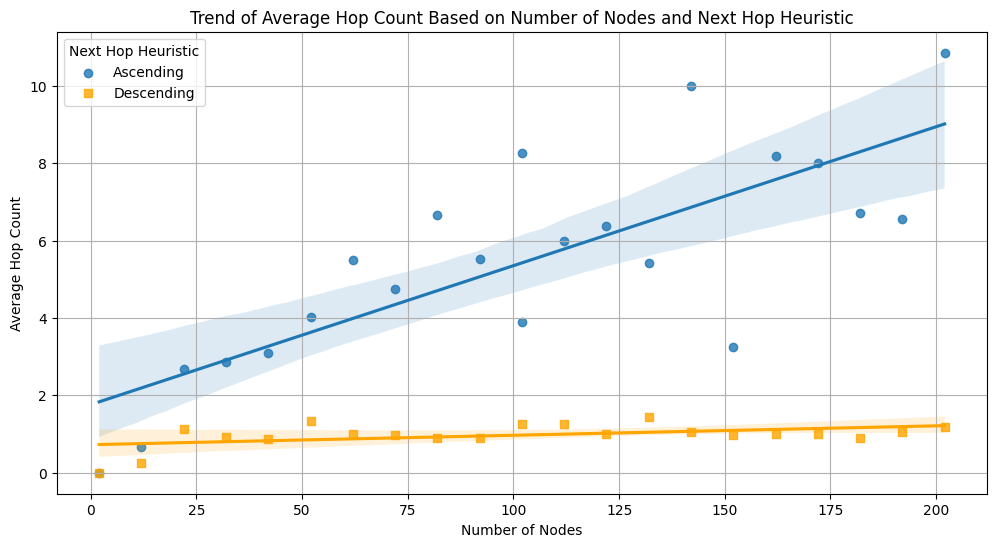
\includegraphics[width=1\linewidth]{images/hop_count.png}
    \caption{Trend of Average Hop Count Based on Number of Nodes and Next Hop Heuristic}
    \label{fig:enter-label}
\end{figure}

The \textbf{Descending} heuristic demonstrates a clear advantage over the \textbf{Ascending} heuristic, which is probably caused by the \textbf{sink} node being assigned the \textbf{highest IP address}, making it more accessible when routing tables prioritize descending IP order. This structure leads to \textbf{more efficient} path selection and reduced hop count, ultimately improving network performance.

\end{document}